% !Mode:: "TeX:UTF-8"
% !TEX program  = xelatex
\documentclass[a4paper]{article}
\usepackage{amsmath}
\usepackage{amssymb}
\usepackage{ctex}
%\usepackage{braket}
%\usepackage[european]{circuitikz}
\usepackage{multirow}
\usepackage{float}
\usepackage{graphicx}
\usepackage{geometry}
\geometry{left=2.5cm,right=2.5cm,bottom=2.5cm,top=2.5cm}

\usepackage{textcomp}
\usepackage{physics}

\title{近代物理实验报告5.2:X射线衍射物相分析}
\author{\quad 学号\quad 匡亚明学院}
\date{2019年2月29日}
\begin{document}
%\sloppy
\maketitle
\bibliographystyle{unsrt}
%--------main-body------------

\section{引言}
物相分析中的衍射方法包括X射线衍射、电子衍射和中子衍射三种,其中X射线衍射方法使用最广、最为经常。
%它包括德拜照相法、聚焦照相法和衍射仪法等,本实验重点介绍衍射仪法。

X射线最早由德国科学家W.C. Roentgen在1895年在研究阴极射线发现,具有很强的穿透性,又因X射线是不带电的粒子流,所以在电磁场中不偏转。1912年劳厄等人发现了X射线在晶体中的衍射现象,证实了X射线本质上是一种波长很短的电磁辐射,
%其波长约在10nm到10–2nm之间,
与晶体中原子间的距离为同一数量级,是研究晶体结构的有力工具。
%同年,英国物理学家W.H.Bragg和M.L.Bragg发现X射线衍射Bragg公式,测定了NaCl晶体的结构,开创了X射线晶体结构分析的历史。
\section{实验目的}
\begin{enumerate}
\item 掌握物相定性分析基本方法。
\item 掌握D8 X射线衍射仪的使用。
\end{enumerate}


\section{实验原理}

\subsection{X射线的产生和X射线谱}
实验中通常使用X光管来产生X射线。在抽成真空的X光管内,当由热阴极发出的电子经高压电场加速后,高速运动的电子轰击由金属做成的阳极靶时,靶就发射X射线。靶材料的原子序数愈大,X射线波长愈短,能量愈大,穿透能力愈强。
\begin{figure}[H]
	\centering
	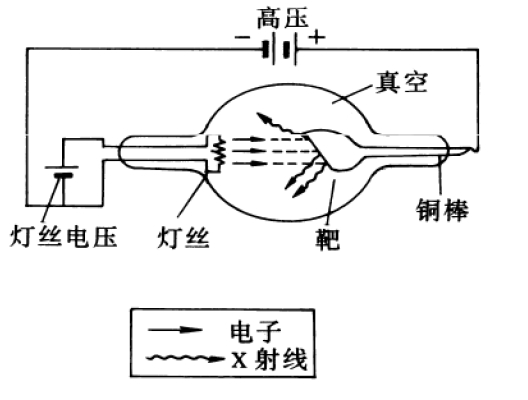
\includegraphics[width=0.5\linewidth]{fig/X1.jpg}
	\caption{X射线管}
\end{figure}

发射出的X射线分为两类:(1)如果被靶阻挡的电子的能量不越过一定限度时,发射的是连续光谱的辐射。这种辐射叫做轫致辐射;(2)当电子的能量超过一定的限度时,可以发射一种不连续的、只有几条特殊的谱线组成的线状光谱,这种发射线状光谱的辐射叫做特征辐射。

对于特征X光谱分为
\begin{itemize}
	\item K系谱线:外层电子填K层空穴产生的特征X射线$ K_\alpha $、$ K_\beta $、...
	\item L系谱线:外层电子填L层空穴产生的特征X射线$ L_\alpha $、$ L_\beta $、...
	\item ...
\end{itemize}
\subsection{X射线与物质的作用}
X射线与物质相互作用产生各种复杂过程。就其能量转换而言,一束X射线通过物质分为三部分:散射,吸收,透过物质沿原来的方向传播,如下图,其中相干散射是产生衍射花样原因。
\begin{figure}[H]
	\centering
	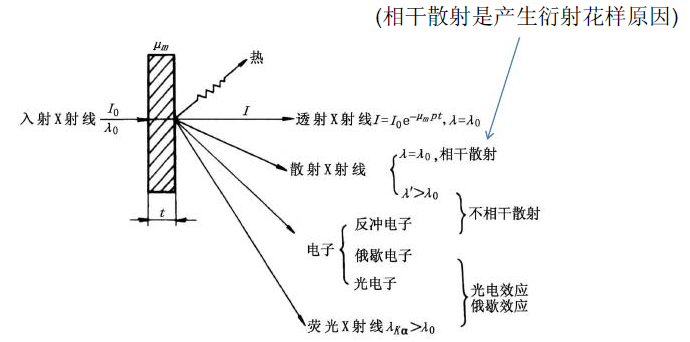
\includegraphics[width=0.7\linewidth]{fig/X2.jpg}
	\caption{X射线与物质的作用}
\end{figure}


\subsection{晶体的X射线衍射}
晶体结构可以用三维点阵来表示。每个点阵点代表晶体中的一个基本单元,如离子、原子或分子等。空间点阵可以从各个方向予以划分,而成为许多组平行的平面点阵。因此,晶体可以看成是由一系列具有相同晶面指数的平面按一定的距离分布而形成的。各种晶体具有不同的基本单元、晶胞大小、对称性,因此,每一种晶体都必然存在着一系列特定的d值,可以用于表征不同的晶体。

X射线波长与晶面间距相近,可以产生衍射。晶面间距d和X射线的波长的关系可以用布拉格方程来表示
\begin{equation}\label{key}
2d\sin\theta = n\lambda
\end{equation}
根据布拉格方程,不同的晶面,其对X射线的衍射角也不同。因此,通过测定晶体对X射线的衍射,就可以得到它的X射线粉末衍射图,如下图所示。
\begin{figure}[H]
	\centering
	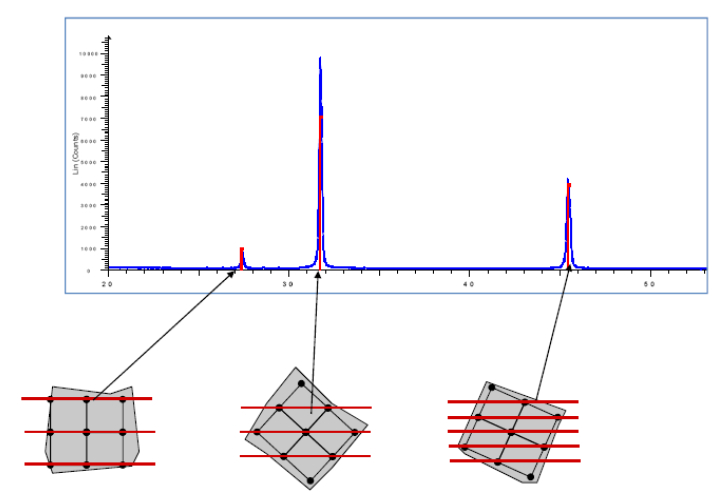
\includegraphics[width=0.85\linewidth]{fig/XRD.jpg}
	\caption{粉末衍射图谱}
\end{figure}

\subsection{物相鉴定原理}
%任何结晶物质均具有特定晶体结构(结构类型,晶胞大小及质点种类,数目,分布)和组成元素。一种物质有自己独特的衍射谱与之对应,多相物质的衍射谱为各个互不相干,独立存在物相衍射谱的简单叠加。
%衍射方向是晶胞参数的函数(取决于晶体结构);衍射强度是结构因子函数(取决于晶胞中原子的种类、数目和排列方式)。任何一个物相都有一套d-I特征值及衍射谱图。因此,可以对多相共存的体系进行全分析。也就是说实验测得的图谱与数据库中的已知X射线粉末衍射图对照,通过两者的匹配性就可以确定它的物相。

任何结晶物质,无论它是单晶体还是多晶体,都具有特定的晶体结构类型、晶胞大小、晶胞中原子、粒子或分子数目的多少,以及它们所在的位置,因此给出特定多晶体X射线衍射花样,更明确地说,一种多晶物质,无论是纯相还是存在于多相混合试样中,它都给出特定的衍射花样、事实上没有两种不同的结晶物质可以给出完全相同的衍射花样。另一方面,未知混合物的花样是混合物中各相物质衍射花样的总和,每种相的各衍射线条的d值、相对强度不变,这就是能用X射线衍射方法作物相定性分析(物相鉴定)的基础。

定性分析的基础方法是将未知物相的衍射花样与已知物质的衍射花样相对照,这种方法是Hanawalt及其合作者首先创建的,起初它们搜集了1000多种化合物的衍射数据作为基本参考。后来,美国材料试验学会和X射线及衍射电子学会在1942年出版了第一组衍射数据卡片,以后逐年增编,到1963年一共出版了13组,后来每年出版一组,并分为有机和无机两部分,称为ASTM卡片,1969年建立了粉末衍射标准联合委员会(简称JCPDS),这个国际性组织,在有关国家相应组织的合作下,编辑出版粉末衍射卡组,简称PDF卡组,为了查寻与未知物质花样对比的卡片,还编制了各种索引。


\section{实验仪器}
德国布鲁克公司D8 X射线衍射仪
\begin{itemize}
	\item X射线光源: 3kW封闭靶(陶瓷X光管)。
	\item 测角仪: 扫描方式$ \theta/\theta $联动测角仪,测角仪的样品台水平放置并保持不动,角度重现性达到$ 0.0001\textdegree $。
	\item 驱动方式:步进马达驱动; 最高定位速度:$ 1500 $\textdegree/min
	\item 狭缝系统:包括索勒狭缝、发散狭缝、防散射狭缝、接受狭缝等。
	\item LynxEye 探测器:(1)强度增益比常规的闪烁计数器高150倍,同时具有优秀的分辨率及信噪比。(2)超快的测量速度。(3)良好的低角度测量性能。(4)良好的分辨率。
	\item 循环水冷系统:要求连续工作; 控温精度$ \leq \pm 2\textcelsius $; 供水流量,满足发生器要求, 进水度可调; 过热保护。
\end{itemize}
\begin{figure}[H]
	\centering
	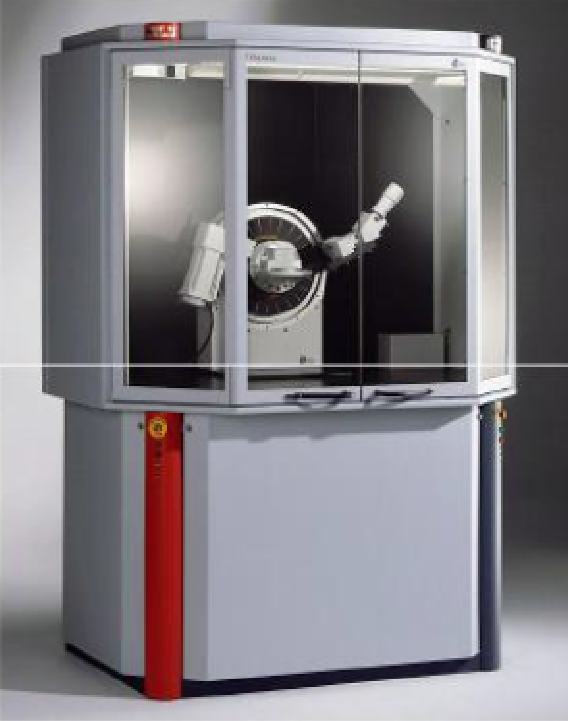
\includegraphics[width=0.55\linewidth]{fig/D8.png}
	\caption{D8 X射线衍射仪}
\end{figure}

\section{实验内容}
\subsection{X射线衍射}
\begin{enumerate}
\item 样品的制备和安装。
\begin{enumerate}
\item 将被测试样放在玛瑙研钵中研磨至200$\sim$300目(本次实验略去这一步)。
\item 把平板玻璃与试样板擦净,试样板放在玻璃上,把有线条一面朝下,用刮刀将粉末填入样品板孔中,略高于样品板,用刮刀将试样压平,勿反复压,也不要拖刮刀。试样压好后,紧贴平板玻璃一面作为X光照射面,并检查一下是否平整。(本次实验略去这一步)
\item 将样品板插入样品台架,其中心线对准样品台的中心线。
\end{enumerate}
\item 按D8 X射线衍射仪操作规程开机。
%选择各参数(时间常数、扫描速度、狭缝宽度、量程等),同时打开记录仪开关,开始测量。即可获得一张衍射图谱。
\begin{enumerate}
	\item 开总电源。
    \item 开电脑。
	\item 开循环水。
	\item 开仪器电源(按绿色按钮,由4灯全亮变成ON和ALARM灯亮)。
	\item 开X-ray高压(右侧扳手顺时针向上扳45度保持$ 3\sim 5 $秒,直到Ready灯亮)。
	\item 开BIAS(在前盖盘内)。
\end{enumerate}
\item 开软件XRD Commander。在XRD Commander里升电压和电流,每隔30秒加5kV直到40kV;然后加电流,每隔30秒加5mA直到40mA。如果停机2天以上最好做光管老化。
%:点击D8 Tools主界面/X-ray generator,点击工具栏里的utilities/X-ray.../Tube condition ON/OFF,在右下角的状态栏出现Tube condition ON,电压和电流会逐步升到50kV-5mA。大概需要1小时,等电压和电流回到20kV-5mA,点击Tube condition ON/OFF老化结束。
\item 在XRD Commander中初始化(点击两个轴上面的选项Requested,选定两个轴,使Tube为20,Detector为20,点击菜单里的初始化图标进行初始化)。做物相分析在Scantype中选Locked Coupled,并且在Detail中将探测器改为1D。
在XRD Commander中选择各参数(起始角、终止角、步长等)开始测量。即可获得一张衍射图谱,将其保存为*.raw文件。\\
对于未知的样品:首先,扫描范围$ 10\textdegree\sim 90\textdegree $,步长大些,快速扫描。然后,参照第前面的谱线,把扫描起始角放在第一个峰前一点,把终止角放在最后一个峰后一点。对于一般定性分析用连续扫描。对于定量分析(例如无标样定量相分析等)对强度要求高,就用步进扫描。
\item 按D8 X射线衍射仪操作规程关机。
\begin{enumerate}
	\item 在软件里降高压。在软件XRD Commander里将高压调到20kV$ \sim $5mA,点击“Set”。
	\item 关软件XRD Commander。
	\item 关X-ray高压(右侧扳手逆时针向上扳45度),再等5分钟。
	\item 关仪器电源(按红色按钮)。
	\item 关循环水(关仪器电源后迅速关水)。
	\item 关BIAS(在前盖盘内)。
	\item 关电脑。
    \item 关总电源。
\end{enumerate}
\end{enumerate}

\subsection{物相分析}
\iffalse
\begin{enumerate}
	\item 根据衍射图谱选出三条最强线$d_1$,$d_2$,$d_3$(按强度减弱排列)。
	\item 根据最强线的面间距$d_1$,在Hanawalt数字索引中找到所属的组,再根据$d_2$和$d_3$找到其中的一行。
	\item 比较此行中的三条线,看其相对强度是否与待测试样的三强线基本一致。如$d$和$\frac{I}{I_1}$都基本一致,则可初步判断未知试样中含有所载的这种物质。
	\item 根据索引中查找的卡片号,从卡片盒中找到所需卡片。
	\item 将卡片上全部$d$和$\frac{I}{I_1}$与未知试样的$d$和$\frac{I}{I_1}$对比,如果完全吻合,则卡片上记载的物质,就是要分析的试样。
\end{enumerate}
实验中得出的$d$和$\frac{I}{I_1}$,与卡片上记载的数据可能有出入,这是由于实验条不同和测量准确度不同所造成。在$d$和$\frac{I}{I_1}$这两组数据中,应以$d$的吻合为主。
\fi
\begin{enumerate}
	\item 打开Eva软件。
	\item 将待处理的数据文件导入。点击File/Import/Scan调入原始数据文件*.raw进行处理(或点击File/Open调入*.EVA文件进行处理)。
	\item 在ToolBox框内进行数据处理。
	\begin{enumerate}
		\item 扣背景:点击Backgnd/点击Default/点击Replace,显示扣背景处理后的数据
		\item 删除k:点击Strip k/点击Default/点击Replace,显示处理后的数据(也可以上下移动滑块调整至合适,单击Replace,显示处理后的数据)
		\item 平滑处理:单击Smooth/点击Default/点击Replace,显示处理后的数据(也可以设定需要平滑的参数,左右或上下移动滑块进行调整,合适后单击Replace,显示处理后的数据)
		\item 寻峰:点击Peak Search,设定寻峰参数(门槛threshold与峰宽Width标定,可以上下移动滑块进行调整)。点击“Append to list”标定全谱衍射d值(标定漏峰只需按左键将“$ \downarrow $”拖移至峰顶点击即可,删除峰可点击删除峰与“$ \cross $”即可),此时数据在peak状态列于框内。
	\end{enumerate}
    \item 选定所有的峰,单击Made DIF生成DIF文件。
    \item 物相的定性分析:点击Search/Match。在Search/Match框内选择前三个Quality Marks,选择可能的元素,并选择Pattern,点击Search进行检索/匹配。(先选Toggle All/点击左上角的元素“H”可以将所有的元素变为红色,即肯定没有。选择肯定有的点成绿色。选择可能有的点成灰色。)。最后根据列表给出的可能物质通过比较卡片内的谱线和实际测量出谱线的吻合程度来确定组成成分,也就完成了X射线衍射的初步分析工作。
    \item 导出分析结果。
\end{enumerate}

\section{实验数据}

\section{误差分析}

\section{思考题}
% 书上:
%\subsection*{定性物相分析的基本方法是什么?}
%\subsection*{XD-3A X射线衍射仪由哪几部分组成?}
%\subsection*{实验中怎样选择时间常数?}
%\subsection*{简述物相分析的步骤。}
%\subsection*{叙述物相定性分析的局限性?如何避免相分析的误判或漏判现象?}
%
% 讲义:
\subsection*{X射线在晶体上产生衍射的条件是什么?}
\subsection*{为什么实验中要首先开启冷却水?}
\subsection*{实验中使用的样品的颗粒度有无要求?为什么?}
\subsection*{X射线晶体衍射仪的测量精度影响最大的部分是什么?}

\section{问答题}
\subsection*{为什么衍射仪法记录的始终是平行于试样表面的晶面的衍射?}
\subsection*{不平行表面的晶面是否也有衍射产生?}
\subsection*{用衍射仪如何区分单晶、多晶和非晶?}

\nocite{jiaocai}
\bibliography{ref}
\end{document}